\documentclass{hebrew-academic-template}

% Add bibliography file
\addbibresource{advanced_references.bib}

% Title page information
\hebrewtitle{בדיקה מקיפה של התבנית האקדמית}
\englishtitle{Comprehensive Test of the Academic Template}
\hebrewauthor{ד"ר סגל יורם}
\date{\textenglish{September 2025}}

\begin{document}

\maketitle

\tableofcontents
\newpage

% ==================== INTRODUCTION ====================

\hebrewsection{מבוא: \entoc{Introduction}}

This section tests basic Hebrew text with English terms like \en{Computer Science} and \en{Artificial Intelligence}. We can also include numbers like \num{123} and years like \hebyear{2025}. Mathematical expressions such as $a^2 + b^2 = c^2$ are also supported.

\hebrewsubsection{מטרות הבדיקה: \entoc{Testing Goals}}

This subsection will test the following features:

\begin{itemize}
    \item Correct rendering of mixed Hebrew and English text.
    \item Proper functioning of citations with LTR numbers \cite{devlin2018bert}.
    \item Correct display of tables and figures.
    \item Verification of code blocks and lists.
\end{itemize}

% ==================== ADVANCED CONTENT ====================

\englishsection{Advanced Content}

This is an example of a section written entirely in English. It can contain citations like \cite{vaswani2017attention} and mathematical formulas such as:

\begin{equation}
    E = mc^2
\end{equation}

This section helps to verify that the template can handle both Hebrew-majority and English-majority documents.

\hebrewsection{תוכן מורכב בעברית: \entoc{Complex Hebrew Content}}

This section includes more complex examples, such as nested lists and more citations \cite{hebrew_nlp_2023,hebrew_linguistics_2022}.

\begin{enumerate}
    \item The first item in a numbered list.
    \item The second item, which contains a nested list:
    \begin{itemize}
        \item A nested bullet point.
        \item Another nested bullet point with an English term: \en{Nested Item}.
    \end{itemize}
    \item The third item in the list.
\end{enumerate}

\hebrewsubsection{טבלה מורכבת: \entoc{Complex Table}}

\begin{hebrewtable}[h]
    \caption{השוואה בין אלגוריתמים: \en{Algorithm Comparison}}
    \begin{rtltabular}{|c|c|c|}
        \hline
        \mixedcell{\textbf{אלגוריתם / \en{Algorithm}}} & \mixedcell{\textbf{סיבוכיות זמן / \en{Time Complexity}}} & \mixedcell{\textbf{סיבוכיות מקום / \en{Space Complexity}}} \\
        \hline
        \en{Bubble Sort} & $O(n^2)$ & $O(1)$ \\
        \hline
        \en{Merge Sort} & $O(n \log n)$ & $O(n)$ \\
        \hline
        \en{Quick Sort} & $O(n \log n)$ & $O(\log n)$ \\
        \hline
    \end{rtltabular}
\end{hebrewtable}

% ==================== CODE AND FIGURES ====================

\hebrewsection{קוד ואיורים: \entoc{Code and Figures}}

\hebrewsubsection{דוגמת קוד ב-Python: \entoc{Python Code Example}}
\begin{pythonbox}[My Python Code]
def fibonacci(n):
    a, b = 0, 1
    while a < n:
        print(a, end=' ')
        a, b = b, a+b
    print()

fibonacci(100)
\end{pythonbox}

\hebrewsubsection{איור לדוגמה: \entoc{Example Figure}}

\begin{figure}[h]
    \centering
    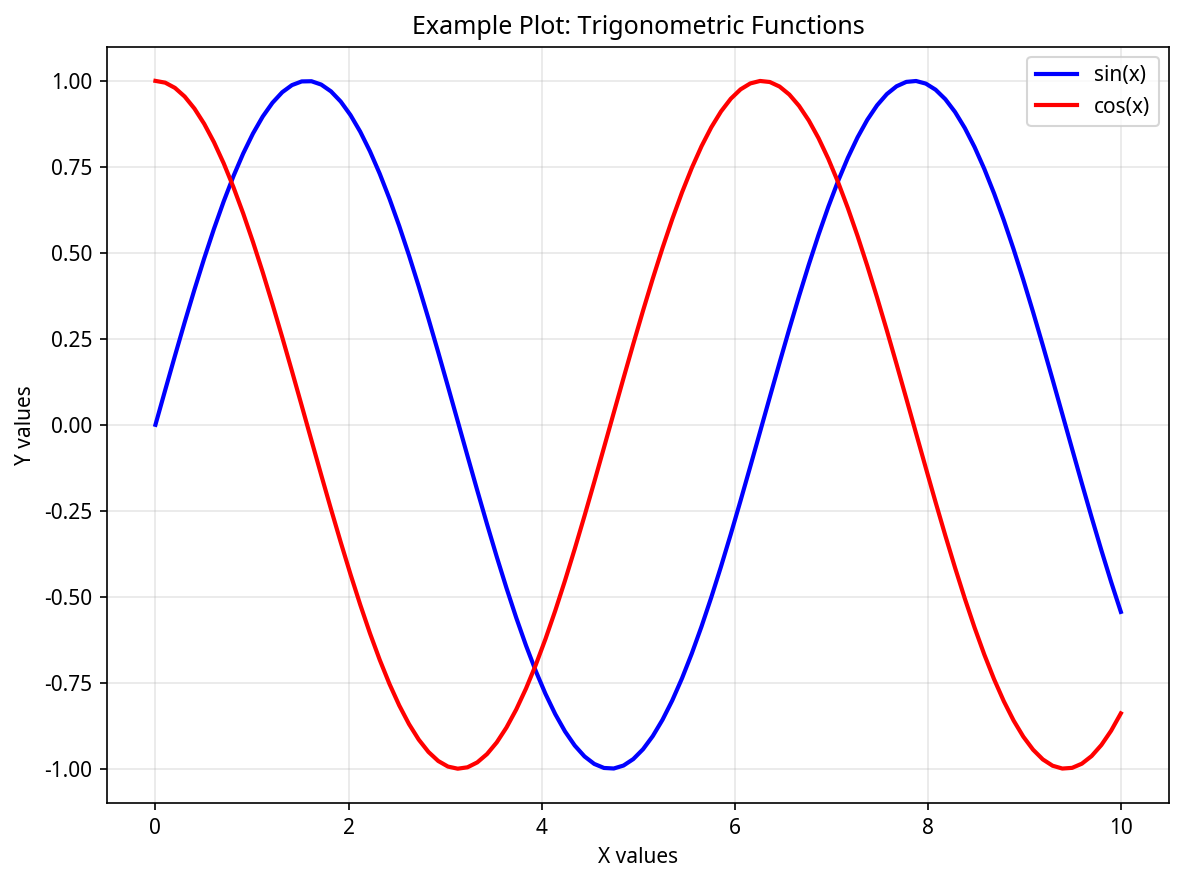
\includegraphics[width=0.6\textwidth]{example_plot.png}
    \caption{גרף לדוגמה: \en{Sample Plot}}
    \label{fig:sample_plot}
\end{figure}

As can be seen in Figure \ref{fig:sample_plot}, the plot shows a simple sine wave.

% ==================== BIBLIOGRAPHY ====================

\newpage
\printhebrewbibliography
\printenglishbibliography

\end{document}

